\begin{exercício}{Condições de contorno para meios lineares}{exercício2}
    Na interface entre dois meios dielétricos, o campo elétrico deve necessariamente ser consistente com as condições de contorno que você resumiu no problema anterior. Assim, considere uma interface genérica entre dois meios \emph{lineares}, como mostra a figura abaixo. As constantes \(\epsilon_1\) e \(\epsilon_2\) correspondem às permissividades elétricas de cada um dos meios e os campos elétricos estão indicados.

    \begin{center}
        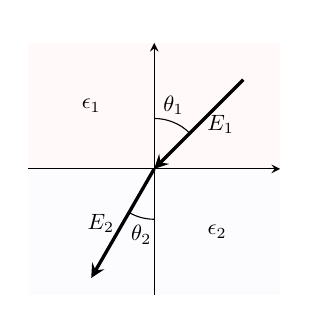
\begin{tikzpicture}[scale = 0.8, every node/.style={scale = 0.8}]
            \fill[Lavender!10] (-2,-2) rectangle (2,0);
            \fill[Pink!10] (-2,0) rectangle (2,2);
            \draw[-stealth] (-2,0) -- (2,0) node[right] {};
            \draw[-stealth] (0,-2) -- (0,2) node[above] {};
            \draw[very thick, stealth-] (0,0) -- +(45:2) node[midway,right] {$\vetor{E}_1$};
            \draw[very thick, -stealth] (0,0) -- +(-120:2) node[midway,left] {$\vetor{E}_2$};
            \draw (0,0.8) arc[start angle=90,end angle=45,radius=0.8] node[midway,above] {\(\theta_1\)};
            \draw (0,-0.8) arc[start angle=270,end angle=240,radius=0.8] node[midway, below] {\(\theta_2\)};
            \node at (-1,1) {$\epsilon_1$};
            \node at (1,-1) {$\epsilon_2$};
        \end{tikzpicture}
    \end{center}

    Prove que se não há cargas livres na interface, então \(\epsilon_2 \tan{\theta_1} = \epsilon_1 \tan{\theta_2}\).
\end{exercício}
\begin{proof}[Resolução]
    Seja \(\vetor{n}\) a normal da interface tal que \(\inner{\vetor{n}}{\vetor{E}_2} = E_2 \cos\theta_2\) e \(\inner{\vetor{n}}{\vetor{E}_1} = E_1 \cos\theta_1\). Se não há cargas livres na interface, então temos \(\epsilon_2 E_2 \cos\theta_2 = \epsilon_1 E_1 \cos\theta_1\). Assim, como \((\vetor{E}_1-\vetor{E}_2)\times\vetor{n} = 0\), segue que \(E_1 \sin\theta_1 = E_2\sin\theta_2\) e então concluímos que
    \begin{equation*}
        \epsilon_2 \tan\theta_1 = \epsilon_1 \tan\theta_2,
    \end{equation*}
    como desejado.
\end{proof}
